% !TeX TS-program = Lualatex
% !TeX encoding = UTF-8 Unicode
% !TeX spellcheck = en
% !BIB TS-program = bibtex
% -*- coding: UTF-8; -*-
% vim: set fenc=utf-8
%%%%%%%%%%%%%%%%%%%%%%%%%%%%%%%%%%%%%%%%%%%%%%%%%%%%%%%%%%%%%%%%%%%%%
% 
\documentclass[runningheads]{llncs}
%
\usepackage[T1]{fontenc}
%
% \usepackage[utf8]{inputenc}
% \usepackage{times}
% \usepackage{wrapfig}
\usepackage{graphicx}
% \usepackage{floatrow}
% \usepackage{multicol}
\usepackage{amssymb}
\usepackage{amsmath}
\usepackage{hyperref}
\usepackage{siunitx}
%%%%%%%%%%%%%%%%%%%%%%%%%%%%%%%%%%%%%%%%%%%%%%%%%%%%%%%%%%%%%%%%%%%%%
% NOTATIONS
% Pixel world
\newcommand{\presynaddr}{a} % pre address
\newcommand{\postsynaddr}{b} % post address
\newcommand{\numevent}{N_{ev}} % total number of events
\newcommand{\presynaddrspace}{\mathcal{A}} %presynaptic address space
\newcommand{\postsynaddrspace}{\mathcal{B}} %postsynaptic address space
\newcommand{\Npol}{N_\text{p}} % number of polarity
\newcommand{\Nneuron}{N_\text{n}} % number of output neurons in the layer
\newcommand{\arank}{r} % address index
\newcommand{\bias}{b} % bias for the MLR model
\newcommand{\synapse}{\mathcal{S}} % synapse
\newcommand{\synapticweight}{w} % synaptic weight
\newcommand{\synapticdelay}{\delta} % synaptic delay
\newcommand{\ranksyn}{s} % synapse index
\newcommand{\Nsyn}{N_{s}} % total number of synapses
\newcommand{\activeweights}{\mathcal{W}} 
\newcommand{\timev}{t} % time
\newcommand{\polev}{p} % polarity
\newcommand{\event}{\epsilon} % event
\newcommand{\eventstream}{\xi} % stream of events
\newcommand{\TS}{S} % time surface
\newcommand{\neuron}{\mathbf{n}} % neuron in the SNN (defined by the spatial position and the channel)
\newcommand{\postneuron}{\mathbf{m}} % post synaptic neuron in the SNN (defined by the spatial position and the kernel)
\newcommand{\channel}{\mathbf{p}} % channel
\newcommand{\layer}{\mathbf{L}} % layer
\newcommand{\ms}{\si{\milli\second}}%
\newcommand{\us}{\si{\micro\second}}%
\newcommand{\timecontext}{T} % time context (cf HOTS) matrice gathering last event times
\newcommand{\current}{I} % post synaptic current
\newcommand{\volt}{u} % membrane potential
\newcommand{\volts}{V} % matrix of membrane potentials
\newcommand{\gain}{\gamma} % homeostatic gain
\newcommand{\simil}{\beta} % similarity value
\newcommand{\Nclass}{N_\text{class}} % number of classes for MLR:
\newcommand{\Nx}{N_\text{X}}
\newcommand{\Ny}{N_\text{Y}}
\newcommand{\Ntime}{N_\text{t}}
\newcommand{\kernel}{K} % convolution kernel
%\newcommand{\kernelind}{\mathbf{k}} % indice of the kernel
\newcommand{\kernelind}{k} % indice of the kernel
\newcommand{\Kx}{K_\text{x}}
\newcommand{\Ky}{K_\text{y}}
\newcommand{\Ktime}{K_\text{t}}
\newcommand{\classiflayer}{\mathbf{C}}
\newcommand{\class}{c} % class k of the MLR
\newcommand{\lrweights}{\theta} % matrix of MLR weights
\newcommand{\lrtrue}{y} % true value of the prediction for MLR
\newcommand{\loss}{J} % cost function for MLR
\newcommand{\softmax}{\sigma}
\newcommand{\actfreq}{f}
\newcommand{\decision}{\hat{y}}
\newcommand{\colorsec}{black}
\newcommand{\colorsubsec}{black}
\newcommand{\speed}{v}
\newcommand{\Nspeed}{N_v}
% Example definitions.
% --------------------
\def\x{{\mathbf x}}
\def\L{{\cal L}}
\newcommand{\fig}[1]{Fig.~\ref{fig:#1}}%{Figure~\ref{fig:#1}}
\DeclareMathOperator*{\argmax}{arg\,max}
\DeclareMathOperator*{\argmin}{arg\,min}

%%%%%%%%%%%%%%%%%%%%%%%%%%%%%%%%%%%%%%%%%%%%%%%%%%%%%%%%%%%%%%%%%%%%%%
% \usepackage{natbib}
% \usepackage[
% %style=chem-acs,
% style=numeric,						% numeric style for reference list
% citestyle=numeric-comp,
% %style=alphabetic-verb,
% giveninits=false,
% maxbibnames=1,
% %firstinits=true,
% %style=apa,
% %maxcitenames=1,
% %maxnames=3,
% %minnames=1,
% %maxbibnames=99,
% dateabbrev=true,
% giveninits=true,
% %uniquename=init,
% url=false,
% doi=false,
% isbn=false,
% eprint=false,
% texencoding=utf8,
% bibencoding=utf8,
% autocite=superscript,boutin_effect_2020
% backend=biber,
% %sorting=none,
% sorting=none,
% sortcites=false,
% %articletitle=false
% ]{biblatex}%

% \bibliography{ref.bib}
%%%%%%%%%%%%%%%%%%%%%%%%%%%%%%%%%%%%%%%%%%%%%%%%%%%%%%%%%%%%%%%%%%%%%%
% \newcommand{\mycaption}[1]{\caption*{#1}}

% \usepackage{titlesec}
% % \titlespacing*{<command>}{<left>}{<before-sep>}{<after-sep>}
% \titlespacing*{\section}
% {0pt}{1.5ex}{0.8ex}
% \titlespacing*{\subsection}
% {0pt}{0.9ex}{0.4ex}
% \titlespacing*{\subsubsection}
% {0pt}{0.5ex}{0.3ex}
% \titlespacing*{\paragraph}{%
%   0pt}{%              left margin
%   0.0\baselineskip}{% space before (vertical)
%   1em}%               space after (horizontal)

% \usepackage{setspace}

\begin{document}

%%%-----------------------------------------------------------------
\title{Accurate detection of spiking motifs in multi-unit raster plots}

\author{Laurent U Perrinet\orcidID{0000-0002-9536-010X}}
%
\authorrunning{LU Perrinet}
% First names are abbreviated in the running head.
% If there are more than two authors, 'et al.' is used.
%
\institute{INT UMR 7289, Aix Marseille Univ, CNRS; 27 Bd Jean Moulin, 13005 Marseille, France
% \url{https://laurentperrinet.github.io} \email{laurent.perrinet@univ-amu.fr}
}
%
\maketitle              % typeset the header of the contribution
%
\begin{abstract} Recently, there has been growing interest in the hypothesis that information may be carried within neural activity by repeating spiking motifs. As a consequence, there has been several recent proposals of algorithms for the detection of such motifs, for instance applied to multi-unit raster plots. In this study, we introduce an extension of such detection models by providing a generative model for raster plot synthesis. An optimal detection procedure is derived from this model. This takes the form of a logistic regression coupled with a temporal convolution. We evaluate the ability of this model to detect spike patterns in synthetic data. Since this model is differentiable, we derive an unsupervised learning method in the form of gradient descent on the loss function of an auto-encoder model for the raster using the spike patterns. This unsupervised learning method is able to recover the synthetically generated spike patterns, and we plan to apply it to neurobiological data as well.
\keywords{Spiking motifs \and heterogeneous delays \and detection.}
\end{abstract}

%----------------------------%
\section{Introduction}
%---------------------------

%%%%%%%%%%%%%%%%%%%%%%%%%%%%%%%%%%%%%%%%%%%%%
\subsection{The age of large-scale neurobiological event-based data}
%%%%%%%%%%%%%%%%%%%%%%%%%%%%%%%%%%%%%%%%%%%%%
% 

TODO read and cite~\cite{mackevicius_unsupervised_2019} wesh

Over the past decade, tremendous technological advances across several disciplines have dramatically expanded the frontiers of experimentally accessible neuroscientific facts. Bridging across different spatial and temporal scales, combination of \textit{in vivo} two photon imaging, large population recording-array technologies, optogenetic circuit control tools, transgenic manipulations as well as large volume circuit reconstructions are now used to examine the function, structure and dynamics of neural networks on an unprecedented level of detail and precision. The daunting complexity of the biological reality revealed by these technologies highlights the importance of neurobiological knowledge to provide a conceptual bridge between abstract principles of brain function and their biological implementations within neural circuits. As a consequence, there is a growing need to scale these methods to larger amounts of data. 

There are multiple approaches which aim at tackling this problem. One algorithm capable of achieving such a daunting task is the Rastermap algorithm~\cite{pachitariu_robustness_2018}. Basically, it rearranges neurons in the raster plot based on the similarity of their activity and applies a deconvolution strategy based on a linear model. Yet this method was mainly tested on calcium imaging data which is known to add some imprecision to the timing of the original spiking activity. The model is openly accessible~\cite{stringer_mouselandrastermap_2020} and has led to important discoveries. In~\cite{stringer_spontaneous_2019} for instance, it was shown that a neuronal population encodes information most efficiently when its stimulus responses are high-dimensional and uncorrelated, and most robustly when they are lower-dimensional and correlated. Then, in~\cite{stringer_high-precision_2021}, the authors analyzed spontaneous neural firing, finding that neurons in the primary visual cortex encoded both visual information and motor activity related to facial movements. In~\cite{russo_cell_2017}, the authors developed novel machine learning tools and statistical tests for unsupervised spatio-temporal pattern detection in non-stationary environments, which were applied to simultaneous electro-physiological recordings from tens to hundreds of neurons for decoding cognitive processes from neural activity. Altogether, this provides evidence for the importance of such machine-learning-based tools to provide with breakthroughs in neuroscience.

In the paper by~\cite{russo_cell_2017}, the authors present a unifying methodological and conceptual framework which detects assembly structure at many different time scales, levels of precision, and with arbitrary internal organization. It uses  sliding window as in~\cite{grun_unitary_2002} and the reliable and efficient analysis of an excess or deficiency of joint-spike events~\cite{pipa_neuroxidence_2008}. They extend the measure to multiple lags~\cite{torre_synchronous_2016}. The core measure is based on a non-stationarity corrected parametric statistical test for assessing the independence of pairs and an agglomerative, heuristic clustering algorithm for fusing significant pairs into higher-order assemblies.  To overcome the limits of models which either require spike times to be discretized, utilize a suboptimal least-squares criterion, or do not provide uncertainty estimates for model predictions or estimated parameters, Williams {\it et al}~\cite{williams_point_2020} address each of these shortcomings by developing a point process model that characterizes fine-scale sequences at the level of individual spikes and represents sequence occurrences as a few marked events in continuous time. As originally introduced by~\cite{kass_statistical_2005}, they use learnable time-warping parameters to model sequences of varying duration, which have been experimentally observed in neural circuits, and demonstrate these advantages on experimental recordings from songbird higher vocal center and rodent hippocampus. Building such models for predicting changes of timings based on context, such as using a so-called change point model for blocked-based experimental protocols~\cite{pasturel_humans_2020}, could therefore provide useful prior information to enhance the decoding from neural activity.
%
%%%%%%%%%%%%%%%%%%%%%%%%%%%%%%%%%%%%%%%%%%%%%
\subsection{Decoding neural activity using spike distances}
%%%%%%%%%%%%%%%%%%%%%%%%%%%%%%%%%%%%%%%%%%%%%
There are different solutions to provide with a distance between two given spike trains. A known measure is the Victor-Purpura distance, which overcomes inconsistencies experienced with a firing rate (Poisson model) of spike trains~\cite{victor_nature_1996}. Then a study tries to solve the problem by including a time constant as a parameter~\cite{van_rossum_novel_2001}. This parameter will then be used to interpolate the distance between a coincidence detector and a rate difference counter. Such distances were extended to non-Euclidean metrics and use morphological manipulations to compute spike train dissimilarity~\cite{kreuz_measuring_2007}. Mathematically, the stability of distance measures induced by level-crossing sampling can be evaluated~\cite{moser_stability_2014}, notably in light of the so-called Weyl's discrepancy measure~\cite{weyl_ueber_1916}, which may lead to the definition of a cross-correlation measure. An interesting conclusion since cross-correlation measure isadapted to the event-based nature of spiking signals. These observations lead to the intuition that each distance may be as well  as the optimal solution of a generative model for these measures, possibly through non-linear relations~\cite{aronov_non-euclidean_2004}. % ~\cite{} 

%Let us now focus on distances defined based on a generative model formed by using precise spiking motifs. 
Concerning spike timings,~\cite{levakova_review_2015} have reviewed existing methods for estimating the latency of neural responses that include Bayesian binning. Alternatively, unitary event analysis can be performed by a statistical model of coincidence detection~\cite{grun_unitary_2002-1}. This was extensively used in detecting above chance significant synchronous patterns~\cite{grun_unitary_2010}, in particular in recordings of pairs of neurons (see~\cite{riehle_spike_1997} for instance), and has been extended to non-stationary data~\cite{grun_unitary_2002}. A method to detect significant patterns of synchronous spiking in a subset of massively parallel spike trains in the presence of background activity can be defined using the statistical evaluation of synchronous spike patterns extracted by frequent item set mining~\cite{torre_statistical_2013}. By the same group, the SPADE, CAD or ASSET algorithms are methods for identification of spike patterns in massively parallel spike trains (the spiking activity of tens to hundred(s) of neurons recorded in parallel) by identifying fine temporal correlations in the$~\ms$ precision range~\cite{quaglio_methods_2018}. This was recently extended in~\cite{stella_3d-spade_2019} in order to find re-occurring patterns in parallel spike train data, and to determine their statistical significance. The extension improves the performance in the presence of patterns with different durations, such as surrogates generated to evaluate precisely timed higher-order spike correlations~\cite{stella_comparing_2022}.

Another important algorithm, called SPOTDisClust, is based on the detection of structured temporal patterns~\cite{grossberger_unsupervised_2018}. They introduced an unsupervised method based for their detection from high-dimensional neural ensembles. The algorithm measures similarity between two ensemble spike patterns by determining the minimum transport cost of transforming their corresponding normalized cross-correlation matrices into each other. Many approaches to this problem are supervised. In other words, they take patterns occurring concurrently with a known event, such as the delivery of a stimulus for sensory neurons or the traversal of a running track for determining hippocampal place fields, as a ``template'' and then search for repetitions of the same template in spiking activity~\cite{nadasdy_replay_1999,lee_combinatorial_2004}. In SPOTDisClust, the learning is unsupervised. It uses the prior that there is only one spike per pattern. Using a so-called t-SNE projection (that allows to project this high-dimensional representation to a lower-dimension map) validated that this clustering method can retrieve all patterns from the data. The limits of this method are that it is computationally complex, block-based and strictly specialized for the task at hand. To overcome these difficulties, a novel method was recently developed~\cite{sotomayor-gomez_spikeship_2021}. Whether it is the distance between two given spike trains or a comparison of the spike timings, the complexity and the diversity of the methods used to measure them are witnesses of the growing interest of the integration of these measures in the understanding of the neural code. One of the steps to test their potential usefulness is then to scale these methods to larger amounts of data.

%
\subsection{Outline}
%%%-----------------------------------------------------------------

As we saw, most SNN, and in particular those adapted from analogous deep-learning-like architectures, rely on an encoding of information based on a continuously varying firing-rate. Notable exceptions of SNNs using precise spike timings are the time encoding machine by~\cite{lazar_time_2004} and \textit{polychronization} model of Izhikevich~\cite{izhikevich_polychronization_2006}. In this section we focus on the polychronization model based on a random recurrent model of spiking neurons including synaptic delays chosen from a range of biologically realistic delays (from $0$ to $20~\ms$) and whose weights evolved with a Spike-Time Dependent Plasticity (STDP) learning rule~\cite{markram_regulation_1997}. It was shown that spike timing (STDP) has an impact on the development of synaptic efficacy for many kinds of neurons~\cite{caporale_spike_2008}. Delays are defined as the total time taken for a spike to be conducted from one presynaptic neuron's soma to the efferent postsynaptic neuron's soma. It is worth mentioning that only the weights are changed using the STDP rule and that the set of delays is set randomly at initialization and that delays are then ``frozen'' for the rest of the simulation. Due to the interplay between the delays and STDP, the spiking neurons spontaneously self-organize into groups and generate patterns of stereotypical polychronous activity, i.e.~exhibit reproducible time-locked firing patterns which  the author defined as ``polychronous groups''. One core ingredient of this model is the fact that the neurons composing a group fire at different times, but due to the heterogeneous delays, the spikes reach the postsynaptic neuron at the same time. This synchrony of arrival at the soma of the neuron leads to the summation of the excitatory post-synaptic potentials evoked by each spike, and thus to the crossing of the voltage threshold and to the discharge of a spike (see Figure~\ref{fig:izhikevich}). According to the STDP rule, the group of neurons involved in this polychronous activity will see their synaptic weight increase and, thus, may consolidate the formation of a polychronous group. 

%----------------------------%
%
\begin{figure}[t]
  \centering
  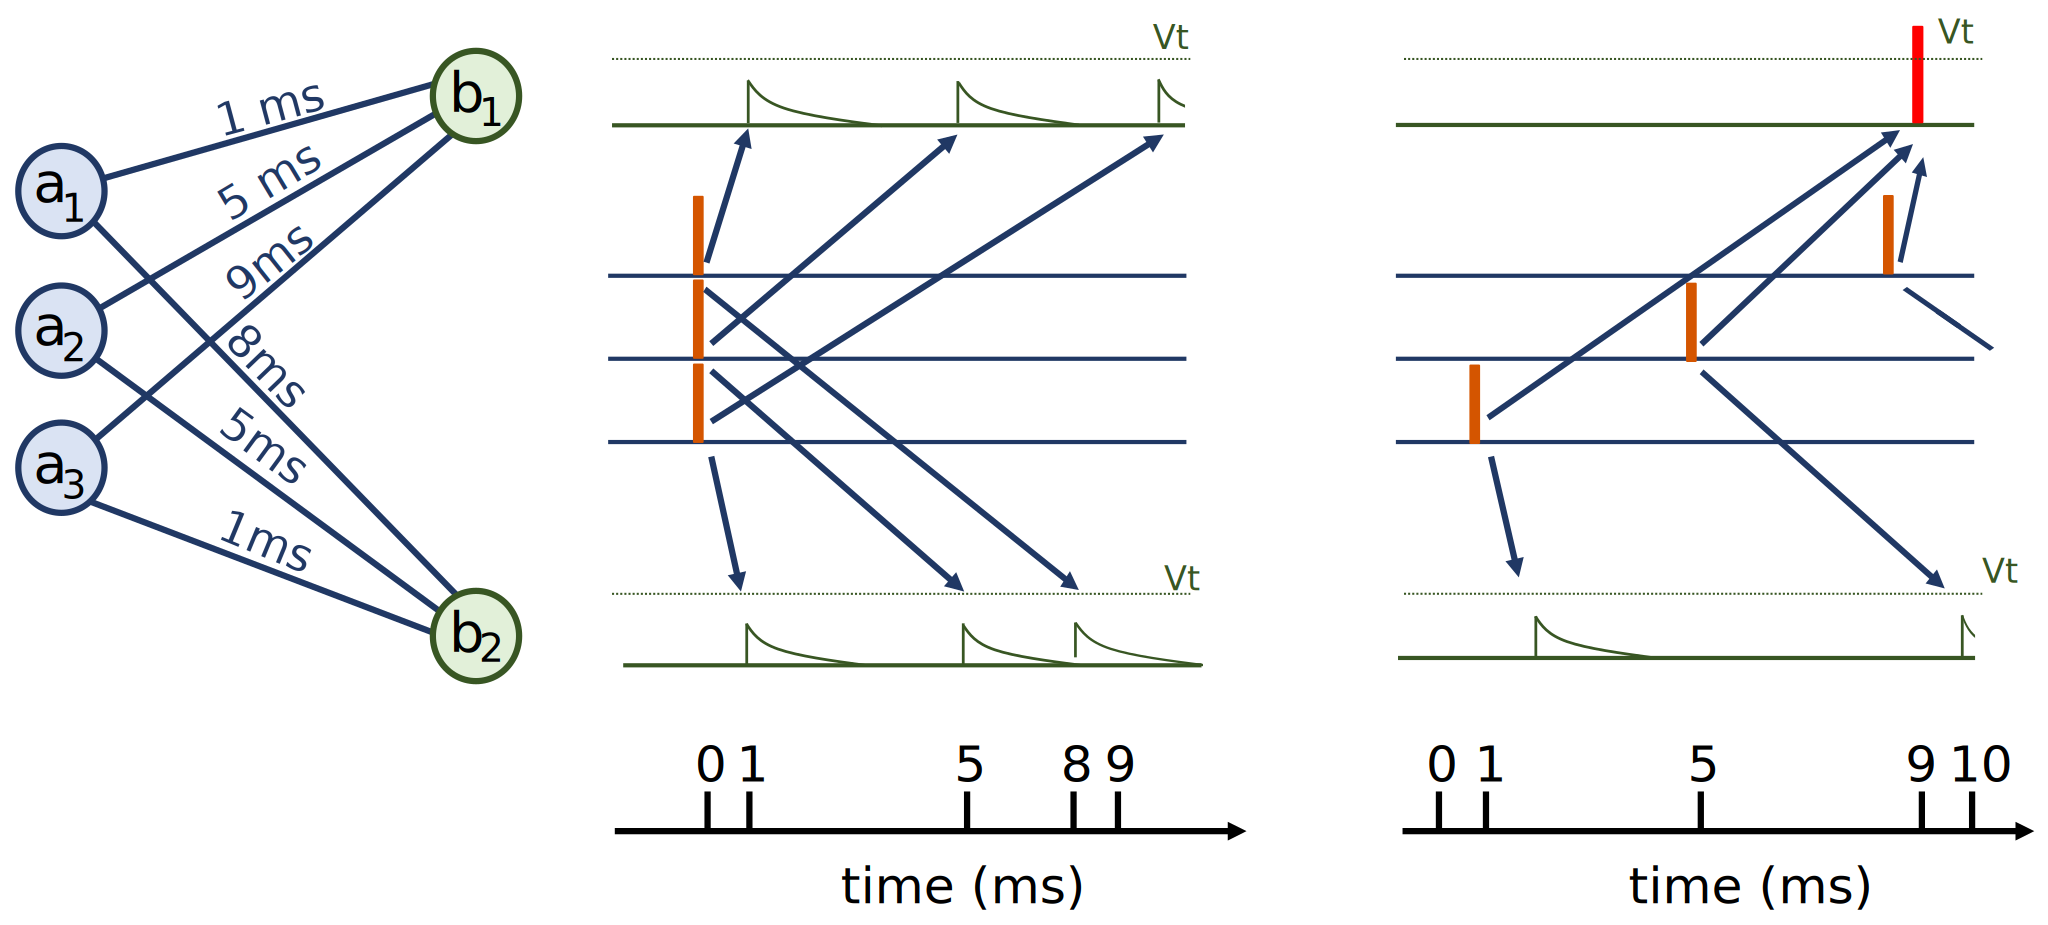
\includegraphics[width=0.80\linewidth]{figures/izhikevich.pdf}%png}% https://www.overleaf.com/5625872443qpcwrkssgbsf
    \caption{\textbf{Core mechanism of polychrony detection~\cite{izhikevich_polychronization_2006}.} \textit{(Left)}~In this example, three presynaptic neurons denoted \textit{b}, \textit{c} and, \textit{d} are fully connected to two post-synaptic neurons \textit{a} and \textit{e}, with different delays of respectively $1$, $5$, and $9~\ms$ for \textit{a} and  $8$, $5$, and $1~\ms$ for \textit{e}. \textit{(Middle)}~If three synchronous pulses are emitted from presynaptic neurons, this will generate post-synaptic potentials that will reach \textit{a} and \textit{e} asynchronously because of the heterogeneous delays, and they may not be sufficient to reach the membrane threshold in either of the post-synaptic neurons, therefore no spike will be emitted as this is not sufficient to reach the membrane threshold of the post synaptic neuron, so no output spike is emitted.
    %at these different delays, and these may not be sufficient to generate a spike in either neuron.
    \textit{(Right)}~If the pulses are emitted from presynaptic neurons such that, taking into account the delays, they reach the post-synaptic neuron \textit{a} at the same time (here, at $t=10~\ms$),  the post-synaptic potentials evoked by the three pre-synaptic neurons sum up, causing the voltage threshold to be crossed and thus to the emission of an output spike (red color), while none is emitted from post-synaptic neuron \textit{e}.
     }
  \label{fig:izhikevich}
\end{figure}
%----------------------------%

In this work, we propose to accurately detect spatio-temporal spiking motifs using a single layer of spiking neurons equipped with heterogeneous delays (HD-SNN). The paper is organized as follows. We develop a theoretically defined HD-SNN for which we can attune both the weights and delays. We first detail the methodology by defining the basic mechanism of spiking neurons that utilize heterogeneous delays. This will allow us to formalize the spiking neuron used to learn the model's parameters and test its effectiveness. In the results section, we will evaluate on a synthetic event-based dataset and show in particular the similarities with neurobiological observations. We will also study the robustness of the spiking motif detection mechanism and in particular its resilience to changing the dimensions of presynaptic, postsynaptic neurons, or the depth in the number of different possible delays. This will allow us to show how such a model can provide an efficient solution which may be applied to neurobiological data.  Finally, we will conclude by highlighting the main contributions of this paper, while defining some limitations. This will open perspectives for future SNNs.  In particular, as neuromorphic devices are by design good candidates for integrating computations over time, we highlight the fact that this event-driven algorithm is perfectly fit to be transferred to this type of hardware and to obtain significant gains in the energy which is used.
%
\section{Methods}
\label{sec:methods}
%%%-----------------------------------------------------------------
%%%-----------------------------------------------------------------
Let us now formally define the Heterogeneous Delays Spiking Neural Network (HD-SNN) model, as well as the task and how we will learn to solve it. First, we will define the model for the efficient detection of event-based motifs using a feed-forward layer of spiking neurons with heterogeneous delays. Our HD-SNN model will be tested on synthetically generated raster plots. By analogy with biological conditions, we will design a paradigm simulating different parameterizations of the raster plot. The task is thus to detect the spiking motifs as accurately as possible. We will describe a detection mechanism for weights and delays. To this end, we will extend the HD-SNN model to be efficient for the resolution of the task by including spatio-temporal convolutional kernels. We will finally describe its implementation on conventional computers. 
%
\subsection{A generative model for raster plots}
%
In neurobiological recordings or in the sensory signal obtained from an event-based camera, any generic raster plot consists of a stream of \emph{spikes}. This can be formalized as a list of neural addresses and timestamps tuples $\event = \{(\presynaddr_\arank, \timev_\arank)\}_{\arank \in [1,\numevent]}$ where $\numevent \in \mathbb{N}$ is the total number of events in the data stream and the rank $\arank$ is the index of each event in the list of events. Events are typically ordered by their time of occurrence. Each event has a time of occurrence $\timev_\arank$  and an associated address $\presynaddr_\arank$ (which is typically in the form $(x_\arank, y_\arank, \polev_\arank)$ for event-based cameras). This defines an address space $\presynaddrspace$ which consists of the set of possible addresses. In a neurobiological recording, this can be the identified set of neurons. %For event-based cameras, it is denoted by $[1, \Nx]\times[1, \Ny] \times [1, \Npol] \subset \mathbb{N}^3$ where $(\Nx, \Ny)$ is the size of the sensor in pixels and $\Npol$ is the number of polarities ($\Npol=2$ for the ON and OFF polarities coded in event-based cameras). 

This raster plot is generated by spiking neurons which are defined on the one hand by the equations governing the evolution of its membrane potential dynamics on its soma and on the other hand by the characterization of the synaptic contacts on its dendritic tree, or on the sensory processes (such as the pixel on the sensor of a camera, or the photoreceptors in the retina). A classical characterization consists in detailing the synaptic weights of each synaptic contact on the dendritic tree, the so-called weight matrix. A more detailed description of these synaptic contacts reveals the added importance of heterogeneous delays, i.e., the precise timing from one afferent neuron's firing to its arrival in the soma, and how this changes the network's dynamics~\cite{izhikevich_polychronization_2006}. In that description, we can parameterize each neuron by the set of tuples defining both the weight and the delay of each synaptic contact. As a consequence, a set of input presynaptic spikes $\event$ will be processed by the dendrites defined by this synaptic set and notably by the respective delays, which will multiplex in time all events. 

Let's formalize a layer of spiking neurons with heterogeneous delays (HD-SNN). Each neuron $\postsynaddr \in \postsynaddrspace$  connects to presynaptic afferent from $\presynaddrspace$. In biology, a single cortical neuron has generally several thousands of synapses. Each synapse may be defined by its synaptic weight and its delay, that is, the time it takes for one spike to travel from the presynaptic neuron's soma to that of the postsynaptic neuron. A postsynaptic neuron $\postsynaddr \in \postsynaddrspace$ is then described by the synaptic weights connecting it to a presynaptic afferent from $\presynaddrspace$ but also by the set of possible delays. Note that a neuron may contact an afferent neuron with multiple different delays. Scanning all neurons $\postsynaddr$, we thus define the full set of $\Nsyn$ synapses, 
as  $\synapse = \{(\presynaddr_\ranksyn, \postsynaddr_\ranksyn, \synapticweight_\ranksyn, \synapticdelay_\ranksyn)\}_{\ranksyn \in [1,\Nsyn]}$, where each synapse is associated to a presynaptic address $\presynaddr_\ranksyn$, a presynaptic address $\postsynaddr_\ranksyn$,  a weight $\synapticweight_\ranksyn$, and a delay $\synapticdelay_\ranksyn$. This defines the full connectivity of the HD-SNN model. Of interest is to define the receptive field of a postsynaptic neuron $\synapse^\postsynaddr =  \{(\presynaddr_\ranksyn, \postsynaddr_\ranksyn, \synapticweight_\ranksyn, \synapticdelay_\ranksyn) \| \postsynaddr_\ranksyn=\postsynaddr\}_{\ranksyn \in [1,\Nsyn]} $, or the emitting field of a presynaptic neuron $\synapse_\presynaddr =  \{(\presynaddr_\ranksyn, \postsynaddr_\ranksyn, \synapticweight_\ranksyn, \synapticdelay_\ranksyn) \| \presynaddr_\ranksyn=\presynaddr\}_{\ranksyn \in [1,\Nsyn]}$. As a consequence, an event stream which evokes neurons in the presynaptic address space is multiplexed by the synapses into a new event stream which is defined by the union of the sets generated by each emitting field from the presynaptic space: 
$ \cup_{\arank \in [1,\numevent]} \{ \{(\postsynaddr_\ranksyn, \synapticweight_\ranksyn, \timev_\arank + \synapticdelay_\ranksyn) \}_{ \ranksyn \in \synapse_{\presynaddr_\arank}} \}$. This new stream of events is by nature ordered in time as events reach the soma of post-synaptic neurons. In particular, when post-synaptic neurons are activated on their soma by this spatio-temporal motif, the discharge probability will increase, notably when these spikes converge on the soma in a synchronous manner. 
% \note{ TODO: show why this formula implements a polychrony detector }

% \note{ éclaircir }

Taking the argument the other way around, one may form a generative model for realistic raster plots. Indeed, any spike in the presynaptic address space is generated by sensory neurons (for instance photoreceptors in the retina, sensors in a CMOS chip) or by afferent spiking neurons. In the latter case, these are connected to the spiking cell by a set of weights and delays, whose structure is stable relatively to the coding timescale. When these connections are high and sparsely distributed, this firing will cause a specific temporal motif. Another example is given for the barn owl auditory system: As it hears the sound of a mouse, this sound will generate a specific spiking response in both ears, and specifically, the precise timing between the signal generated by the left relative to the right ear can be for instance used to determine the position of the prey~\cite{goodman_spike-timing-based_2010}. Overall, these examples show that raster plots may be considered as a mixture of the effects of different elementary causes, and that each event triggers a specific spatio-temporal spiking motif. 
%
\subsection{Detecting spiking motifs}
%: Detection model

From the perspective of simulating such event-based computations on standard CPU- or GPU-based computers, it is useful to transform this event-based representation into a dense representation. Indeed, we may transform any event-based input as the boolean matrix $A \in \{0, 1 \}^{N\times T}$, where $N$ is the number of neurons in $\presynaddrspace$ and $T$ is the number of time bins. In this simplified model, we will consider that heterogeneous delays are limited in range such that the synaptic set can be represented by the dense matrix $\kernel^\postsynaddr$ giving for each neuron $\postsynaddr$ the weights as a function of presynaptic address and delay: $\forall {\ranksyn \in [1,\Nsyn^\postsynaddr]}, \kernel^\postsynaddr(\presynaddr_\ranksyn^\postsynaddr, \synapticdelay_\ranksyn^\postsynaddr) = \synapticweight_\ranksyn^\postsynaddr$. 
The probability of firing of a neuron $a$ at a given time $t$ can be understood as a Bernoulli trial whose (only) parameter is a bias $p(t, a) \in [0, 1]$. Assuming that the presence of spiking motifs conditions the probability on all efferents, the logit (inverse of the sigmoid) of this probability bias can be written as the sum of the logit of each of these factors, whose values are defined by the corresponding weights. Spiking motifs may be activated independently and at random times, such that  we write this activity as $B(b, t)=1$ if $b$ is activated at $t$ and else $B(b, t)=0$. We can thus write the probability bias as the accumulated evidence given these factors as 
\begin{equation*}
p(t, a) = \sigma\big(W_0 + \sum_{b, t} B(b, t) \cdot W_b(a, t-d) \big)  
\end{equation*}
where $\sigma$ is the sigmoid function. We will further assume that the weights are balanced (their mean is zero) and that $W_0$ is a bias such that $p_0=\sigma(W_0)$ is the average background firing rate. Conveniently, one can write this summation as a one-dimensional temporal convolution operator such that we may simply write
\begin{equation*}
p = \sigma(W_0 + B \ast W )
\end{equation*}
where  $p\in [ 0, 1]^{N\times T}$ and $B\in \{0, 1\}^{M\times T}$ is the raster plot corresponding to the temporal activation of the spiking motifs. Finally, we obtain the raster plot $A\in \{0, 1\}^{N\times T}$ by drawing spikes using independent Bernoulli trials $A \sim \mathcal{B}(p)$. Note that, depending on the shape of the kernels, the generative model can model a discretized Poisson process, generate rhythmic activity or more generally propagating waves. This formulation thus defines a simple generative model for raster plots as a combination of independent spiking motifs. 
%
%\subsection{Detecting event-based motifs using spiking neurons with heterogeneous delays}
%
%By discretizing time (here with an arbitrary time unit $1~\ms$), we can also define the motifs as a matrix giving the weight with respect to the different delays $d \in [0, D]$ (where $D$ is the maximum delay) at different addresses $a \in [1, N]$ where $N$ is the number of neurons from the multiunit recording. When a given motif is activated, it will produce a discharge pattern corresponding to that specific set of delays and addresses. Let's define the probability of firing of a neuron $a$ at a given time $t$ as a Bernoulli trial whose (only) parameter is a bias $p(t, a) \in [0, 1]$. For any given probability $p$ it is convenient to define the corresponding \emph{evidence} which corresponds to the log odds $\log \frac{p}{1-p} = \sigma^{-1}(p)$, where $\sigma$ is the sigmoid function. Assuming that the presence of spiking motifs is binary, it is easy to show that the total evidence can be written as the sum of these evidences, whose values are given by the corresponding weights. Assuming that we know that there are $M$ such motifs, we define $b \in [1, M]$ the address of a motif and $W_b$ the corresponding weight matrices. This allows us to derive a generative model for raster plots (see \fig{THC}). 
%
 %Spiking motifs may be activated independently at random times and we write that $B(b, t)=1$ if $b$ is activated at $t$ (and otherwise $B(b, t)=0$). We can thus write the probability bias as the joint probability given these factors as $p(t, a) = \sigma\big(W_0 + \sum_{b, t} B(b, t) \cdot W_b(a, t-d) \big)$. We will further assume that the weights are balanced (their mean is zero) and that $W_0$ is a bias such that $p_0=\sigma(W_0)$ is the average background firing rate. Conveniently, this summation can be written as a one-dimensional temporal convolution operator, so we can simply write $p = \sigma(W_0 + B \ast W )$ where  $p\in [ 0, 1]^{N\times T}$ and $B\in \{0, 1\}^{M\times T}$ is the raster plot corresponding to the temporal activation of the spiking motifs. Finally, we obtain the raster plot $A\in \{0, 1\}^{N\times T}$ by drawing spikes using independent Bernoulli trials $A \sim \mathcal{B}(p)$. Note that, depending on the shape of the kernels, the generative model can model a Poisson process, generate rhythmic activity or more generally propagating waves. This formulation thus defines a simple generative model for raster plots as a combination of independent spiking motifs. 
%Using this dense representation, the counting defined above becomes:
%\begin{equation*}
%\mathcal{C}^\postsynaddr(a,t)
%= \sum_{\presynaddr, \synapticdelay_\ranksyn^\postsynaddr} \kernel^\postsynaddr(\presynaddr_\ranksyn^\postsynaddr, \synapticdelay_\ranksyn^\postsynaddr) \cdot A(\presynaddr, \timev-\synapticdelay_\ranksyn^\postsynaddr)
%\end{equation*}
%%
%This shows that $\mathcal{C}^\postsynaddr$ is a temporal convolution of the dense representation of the event stream with the dense kernels formed by the set of synapses:  $\mathcal{C}^\postsynaddr = \kernel^\postsynaddr \ast A$.
%This well-known computation defines a time-invariant, differentiable measure which is very efficiently implemented for GPUs and which we will use for learning the classification of different motifs in the event stream.
%%
%
%\note{formalize the following:}
%More generally, every cause may be considered as occurring independently and one might write the generative model for the generation of the presynaptic events as:
%
%
%Using this formalization, one might now deduce an optimal algorithm for the detection of such temporal motifs.
%
%
%By discretization of time (with here an arbitrary unitary time unit), we can also define the dendrite as a matrix giving the weight corresponding to the different delays $d \in [0, D]$ (where $D$ is the maximum delay) on different pre-synaptic addresses $a \in [1, N]$ defining the list of the $N$ dendrites. We will denote as $W(a, d)$ these weights.
%
%
%Following the observations of~\cite{izhikevich_polychronization_2006}, let us assume that such precise discharge motif defines a polychronous group (PG). Assuming that we know there exists $M$ such groups, we will define as $b \in [1, M]$ the address of a PG and as $W_b$ the corresponding weight matrices. This allows then to derive a generative model for raster plots (\fig{model}-(b)).

% 
This generative model defined above allows to determine this inference model for guessing sources $B$ when observing a raster plot $A$. This assumes that we know the spiking motifs as defined by the $W_b$ matrices. The underlying metric is the binary cross-entropy, as used in the logistic regression model. In particular, if we consider kernels with similar decreasing exponential time profile, we can prove that this is similar to the method of~\cite{berens_fast_2012}. In our specific case, the difference is that the regression is performed in both dendritic and delay space by extending the summation using a temporal convolution operator. Using this forward model, it is possible to estimate the logit (inverse of a sigmoid) $\hat{B}(b, t)$ for the presence of a PG of address $b$ and at time $t$ by using the transpose convolution operator. Equivalently, this consists in using the emitting field $\synapse_\presynaddr$ of presynaptic neurons in place of the receptive field $\synapse^\postsynaddr$ of postsynaptic neurons. It thus comes that when observing $A$, then one may infer $\hat{B} = A \ast W^T$ and select the most activated items. This assumption hold as long as the kernels are uncorrelated, a condition which is met here numerically by chosing a relatively sparse set of synapses (approximately $1\%$ of active synapses).

%---------------------------
\begin{figure}[h!]
    \includegraphics[width=.50\linewidth]{figures/THC_1a_k.pdf}
    \includegraphics[width=.46\linewidth]{figures/THC_1b.pdf}\\
  \includegraphics[width=.50\linewidth]{figures/THC_1c.pdf}
    \includegraphics[width=.50\linewidth]{figures/THC_1a.pdf}
  
\caption{\textbf{(a)}~As an illustration for the generative model, we draw a multiunit raster plot synthesized from $4$ different spiking motifs and for $10$ neurons. \textbf{(b)}~We show these motifs, each identified at the top by a different color. Each neurons and $71$ different possible delays is assigned the evidence of activation (red) or deactivation (blue). \textbf{(c)}~The activation in time of the different motifs is then used to define a generative model for drawing a raster plot on the multi-unit address space. \textbf{(d)}~By inverting this model, an inference model can be defined for their efficient detection. The original raster plot can be annotated with each identified spiking motif.
}
\label{fig:THC}
\end{figure}%wrapfigure}
%---------------------------

%\subsection{Implementation using spiking neurons with heterogeneous delays}
%
% The activation function of our spiking neural is a softmax function implementing a form of  Multinomial Logistic Regression (MLR)~\cite{grimaldi_robust_2022}, in analogy to a spiking Winner-Take-All network~\cite{nessler_bayesian_2013}. 
%It transforms this list of weights into a probability with the following formula:
%$
%Pr(k=\postsynaddr \; \vert \; \timev) =
%\frac 1 Z
%{\exp  (\mathcal{C}^\postsynaddr(\timev) +\bias^\postsynaddr) }
%$ 
%where $\mathcal{C}^\postsynaddr(\timev) = \sum
%\activeweights^\postsynaddr(t)
%$ is the sum of the synaptic weights and $\bias^\postsynaddr$ is the bias linked to neuron $\postsynaddr$. 
%In particular, we expect that some specific motifs may become tightly synchronized as they reach the basal dendritic tree, leading to a high postsynaptic activity which makes it progressively more likely to generate an output spike.
%%
%
% \note{say that it is effortless in biology but difficult on conventional computers}
% In our MLR model with $\Nclass=\Nspeed$ classes, a probability value is predicted for each event at address $\presynaddr_\arank$ and at time $\timev_\arank$ as a softmax function of the linear combination of the list of events on the basal dendrite of a neuron $\postsynaddr$ in association to a specific class. The linear combination can be defined by a set of synapses $\synapse^\postsynaddr$ as described in the heterogeneous delays model. 
%

\section{Results}
%---------------------------
\begin{figure}%[t!]
  \centering
  \includegraphics[width=0.320\linewidth]{figures/THC_N_PGs.pdf}
  \includegraphics[width=0.320\linewidth]{figures/THC_N_pre.pdf}
  \includegraphics[width=0.320\linewidth]{figures/THC_N_PG_time.pdf}
    \caption{Detecting event-based motifs using spiking neurons with heterogeneous delays. 
Accuracy of detection as a function of  {\bf (Left)}~the number $M$ of kernels, 
    {\bf (Middle)}~the number of presynaptic neurons, {\bf (Right)}~the temporal depth $D$ of kernels among $M=144$ kernels.
    }
  \label{fig:model_results}
\end{figure}
%---------------------------

To quantify the efficiency of this operation, we generated $M=144$ synthetic spiking motifs as random independent kernels over $128$ presynaptic inputs and $D=71$ possible delays. We drew random independent instances of $B$ with a length of $T=1000$ time steps and with on average $1.0$ spike per neuron in each draw. This allowed us to generate raster plots which we use to infer $\hat{B}$. We compute the accuracy as the rate of true positive detections (both for inferring the address and its exact timing) and observe on average $\approx 98\%$ correct detections. We further extended this result by showing how the accuracy would evolve as a function of the number of simultaneous spiking motifs, while keeping the same frequency of occurrence. We show in \fig{model_results}~(a) that the accuracy of finding the right PG is still above $80\%$ accuracy with more than $1364$ overlapping spiking motifs. Moreover, we show in \fig{model_results}~(b) that (with $M=144$ spiking motifs fixed) the accuracy increases notably as the temporal depth $D$ of the PG kernel increased, demonstrating quantitatively the computational advantage of using heterogeneous delays. These results were obtained while assuming that we know $W$. However, this is in general not the case, for instance when observing the raster plot of a population of neurons. In the following, we will define a generic visual task and determine a learning algorithm to solve that challenging task. %Inspired by the k-means algorithm, it is possible to devise a self-supervised learning algorithm. Our preliminary results show that it is possible to retrieve spiking motifs embedded in the data, yet that further analysis is necessary to improve the convergence of the algorithm. In particular, it seems promising to use a sparseness constraint in the inference mechanism such as to remove spurious correlations in the inference.


This generative model allows to derive an inference model for the estimation of sources $B$ when observing a raster plot $A$. 
In our specific case, the difference with~\cite{russo_cell_2017,stella_3d-spade_2019} is that the regression is performed in both dendritic and delay space by extending the summation with a temporal convolution operator. Using this forward model, it is possible to estimate the logit (inverse of a sigmoid) $\hat{B}(b, t)$ for the presence of a motif at address $b$ and time $t$ by using the transpose convolution operator. Thus, when observing $A$, one can infer $\hat{B} = A \ast W^T$ and select the most activated elements. In particular, if we consider weights $W_b$ with similar decreasing exponential time profiles, we can prove that this is similar to finding the tuning function of L-NL neurons, as used in the method of~\cite{berens_fast_2012}.
Assuming that we know the spiking motifs as defined by the $W_b$ matrices, we quantified the accuracy of detecting the occurrence of spiking motifs as the average number of times that the exact address and time were inferred.  
To quantify the efficiency of this operation, we generated $M=55$ synthetic spiking motifs as random independent kernels over $128$ presynaptic inputs and $D=71$ possible delays. We drew random independent instances of $B$ with a length of $T=1000$ time steps and with an average of $2.0$ occurrences each. This allowed us to generate raster plots which we used to infer $\hat{B}$. We compute the accuracy as the rate of true positive detections and observe on average about $98\%$ correct spiking motifs for both address and timing.

We extended this result by showing how accuracy would evolve as a function of the number of simultaneous spiking motifs, while keeping the frequency of occurrence the same. We show in \fig{model_results} that the accuracy of finding the right motif is still above $80\%$ accuracy with more than $1364$ spiking motifs. Moreover, we show in \fig{model_results}-Right that (with $M=55$ spiking motifs fixed) the accuracy increases sharply as the temporal depth $D$ of the spiking motifs is increased. This quantitatively demonstrates the potential of using codes with spiking motifs. 

\section{Discussion}


In this paper, we have introduced a generic SNN using heterogeneous delays and have shown how it compares favorably for a visual motion detection task with a state-of-the-art event-based algorithm used for classification. The learned model bears many similarities with neurobiological anatomical observations but also with the results from behavioral results. % \note{to change if we compare to ghosh instead of HOTs if we follow that route} 
The event-driven computations of our method can be reduced drastically through the pruning of synapses, while maintaining top performance for classification. This shows that we may use the precise timing of spikes to enhance neural computations. 
%
\subsection{Synthesis and main contributions}
%%%-----------------------------------------------------------------
To recap, we have introduced in this paper a SNN model with heterogeneous delays that we have trained and evaluated on a complex motion detection task. The model was defined to optimally detect event-driven spatio-temporal motifs. We have shown that when the model is trained on a dataset of natural images with realistic eye movements, the model learns kernels similar to those found in the early visual cortex of humans for example. We have then shown that the model displays similarities with the responses observed in biology. We have evaluated the computational cost of this model if implemented on neuromorphic hardware, showing that the use of heterogeneous delays may be a frugal computational solution for future neuromorphic hardware, but also a key to understand why spikes represent a universal component of neuronal information processing.

Let us highlight some innovations in the contributions presented in this paper. First, the generic heterogeneous model is formalized from first principles for optimal detection of the event-based spatio-temporal motifs, whereas~\cite{ghosh_spatiotemporal_2019,yu_stsc-snn_2022} use a correlation-based heuristic, which we have observed to be less efficient. Moreover, in comparison to HOTS~\cite{lagorce_hots_2017} the weights are explainable as they directly inform on the logit (inverse sigmoid of the probability) of detecting each spatio-temporal spiking motif. Another novelty is that the model simultaneously learns the weights and the delays, while for example the polychronization model~\cite{izhikevich_polychronization_2006} only learns the weights using STDP while the delays are randomly drawn and their values frozen. Moreover, the model is evaluated on a realistic task, while models such as the tempotron are tested on simplified problems~\cite{gutig_tempotron_2006}. Another main contribution is to provide a model that is suitable for learning any type of spatio-temporal spiking motifs and that can be trained in a supervised way by providing a dataset of supervision pairs. This allows for a more flexible definition of the model using this properly labeled dataset instead of relying on a careful description of the physical rules governing a task, e.g., the luminance conservation principle for motion detection~\cite{benosman_asynchronous_2012,dardelet_event-by-event_2021}.
%


\subsection{Main limits}
%%%-----------------------------------------------------------------
We have identified several limits to our model, which we will now detail. First, the complete framework is based on a discrete binning of time that is incompatible with the continuous nature of biological time. We have used this binning to be able to efficiently implement the framework on conventional hardware, especially GPUs, and in particular to be able to use three-dimensional convolutions. We have tested the effect of the size of the time bin and shown that it has essentially no impact on the results presented in this paper. This is consistent with the relative robustness of other event-based frameworks such as HOTS~\cite{lagorce_hots_2017}, where the accuracy was not affected when the input spikes were subjected to noisy perturbations up to $1~\ms$~\cite{grimaldi_robust_2022}. This suggests the possibility of analytically including a precision term in the temporal value of the input spikes, a mechanism potentially implemented by the filtering that is implemented by the synaptic time constant of about $5~\ms$. Furthermore, it is possible to circonvent the necessity of using a time discretization by using a purely event-based scheme. Indeed, it is not necessary to compute voltage traces between two spikes~\cite{hanuschkin_general_2010} and it is thus possible to define a purely event-based framework. Such an architecture could provide promising speed gains for the calculations. % \note{pourrait parler du poster bernstein? de nadafian?}

Another restriction is that this model is purely feed-forward. Therefore, the spikes generated by the postsynaptic neurons are produced solely on the basis of information contained in the classical receptive field. However, it is well known that neurons in a layer can interact using lateral interactions, for instance in V1 and that this can be the basis for computational principles~\cite{chavane_revisiting_2022}. For example, the combination of neighboring orientations may contribute to image categorization~\cite{perrinet_edge_2015}. Furthermore, neural information is modulated by feedback information, for example to distinguish a figure from its background~\cite{roelfsema_early_2016} and it has been shown that feedback may be essential for building realistic models of primary visual areas~\cite{boutin_sparse_2020,boutin_effect_2020}, Notably to explain non-linear mechanisms~\cite{boutin_pooling_2022}. It is currently not possible to implement these recurrent connections in our implementation (lateral or feedback), mainly due to our use of convolutions. However, the generic theoretical model is able to include them by inserting new spikes into the list of spikes that are reaching pre-synaptic addresses. While this is possible in theory, it needs to be properly adapted in practice so that these recurrent connections do not amplify neuronal activity outside a homeostatic state (through an extinction or explosion of activity).  
% \note{ dire que la prédiction permet de faire de la prediction et que ça explique les résultats de leBec}%~\cite{perrinet_motion-based_2012}

Such recurrent activity would be essential for implementing predictive or anticipatory processes. This is essential in a neural system, as it contains multiple different delays that require temporal alignment~\cite{hogendoorn_predictive_2019}. This has been previously modeled to explain for example the flash-lag illusion~\cite{khoei_flash-lag_2017}. %\note{Say that this could be implemented by properly setting the timing of the label} 
As previously stated, this could be implemented using generalized coordinates (that is variables such as position which are complemented by speed, acceleration, jerk, \ldots) and ``neurobiologically, the application of delay operators just means changing synaptic connection strengths to take different mixtures of generalized sensations and their prediction errors''~\cite{perrinet_active_2014}. Our proposed model using heterogeneous delays provides an alternate and elegant implementation solution to this problem.
%
\subsection{Perspectives}
%%%-----------------------------------------------------------------
% \note{la tache ne met pas en avant les capacites des motifs hetero synaptiques =trop simple et peut se faire en HOTS}
In the definition of our task, we highlighted how the generation of events depends on the spatial gradient in each image. This gradient is defined in both horizontal and vertical dimensions and its maxima are generally oriented. Taken together, these oriented edges form the contours of visual objects in the scene~\cite{koenderink_representation_1987}. Thus, there is a dependence within the event stream between motion and orientation information. It would be crucial to study this interdependence further. This could be initiated by training the model on a dataset with labels providing local orientation. %\note{we can say we tried and that it works well}. 
Studying this dependence will allow us to dissociate these two forms of visual information and to enable us to integrate them. In particular, it will allow us to consider that the definition of motion is more accurate perpendicular to an oriented contour (aka, the aperture problem), thus allowing us to implement recurrent predictive rules, such as those identified to dissociate this problem~\cite{perrinet_motion-based_2012}.

The model is trained on a low-level local motion detection task, and one might wonder if it could be trained on higher-level tasks. An example task would be depth estimation in the visual scene. There are multiple sources of information for inferring depth, such as binocular disparity or changes in texture or shading, but in our case, motion parallax would be the most significant cue~\cite{rogers_motion_1979}. This is because objects close to an observer move relatively faster on the retina than an object at a great distance, and also that visual occlusions depend on depth ordering. Using this information, one can segment objects and estimate their depth~\cite{yoonessi_contribution_2011}. However, this would require computing first the optical flow, that is extending the framework described here for a rigid full-field motion to a more generic one where motion may vary in the visual field. A possible implementation is therefore to add a new layer to our model, in analogy with the hierarchical organization highlighted in the visual cortex. This is theoretically possible by using the output of our model (which estimates velocity in retinotopic space) as input to a new layer of neurons that would estimate velocity in the visual field, including the depth dimension in the output supervision labels. This could have direct and important applications, for example in autonomous driving, to detect obstacles in a fast and robust way. Another extension would be to actively generate sensor movements (physically or virtually) to yield better depths estimates, notably to disambiguate uncertain estimates~\cite{nawrot_eye_2003}.

In conclusion, the model we have presented provides a way to efficiently process event-based signals. We have shown that we can train the model in a semi-supervised manner, knowing \emph{what} output label but not knowing \emph{when} it occurs. Another perspective would be to extend the model to a fully self-supervised learning paradigm, i.e., without any labeled data~\cite{barlow_unsupervised_1989}. This type of learning is thought to be predominant in the central nervous system and, assuming that the signal is sparse~\cite{olshausen_emergence_1996}, one could extend those Hebbian sparse learning schemes to spikes~\cite{perrinet_emergence_2004,masquelier_competitive_2009}. We anticipate that this would be particularly well suited to the exploration of neurobiological data. In fact, there is a substantial literature indicating that brain dynamics often organize into stereotyped sequences such as synfire chains~\cite{ikegaya_synfire_2004}, packets~\cite{luczak_sequential_2007}, or hippocampal sequences~\cite{pastalkova_internally_2008,villette_internally_2015}. These motifs are stereotypical and robust, as they can be activated in the same motif from day to day~\cite{haimerl_internal_2019}. In contrast to conventional methodologies that are used to process neurobiological data, such a event-based model would be able to answer key questions regarding the representation of information in neurobiological data. Furthermore, it would open up possibilities in the field of machine learning, especially in computer vision, to address current key concerns such as robustness to attacks, scalability, interpretability, or energy consumption.
% learning
These coding results were obtained under the assumption that we know $W$. However, this is generally not the case, e.g. when looking at the neurobiological raster plot of a population of neurons. Inspired by the k-means algorithm, it is possible to develop a self-supervised learning algorithm for the automatic detection of spiking motifs. For this, we have drawn a random realization for $W$ and defined an auto-encoder scheme that, for each raster plot $A$, infers the sources $B$ and then re-synthesizes the corresponding raster plot. A natural metric is binary cross-entropy, as used in the logistic regression model, and since the model is differentiable, we optimized $W$ using gradient descent (code implemented using the pyTorch library, with an Adam optimizer and a learning rate of $.001$ for $2^{14}$ steps). We used a homeostatic regularization on the average firing rate of $B$ to ensure that each motif was \emph{a priori} equally activated. Our preliminary results show that it is possible to retrieve spiking motifs embedded in synthetic data. However, further analysis is needed to improve the convergence of the algorithm and to apply such algorithms to neurobiological data. %In particular, it seems promising to use a sparseness constraint in the inference mechanism such as to remove spurious correlations in the inference.
%

\subsubsection{Acknowledgements} LP received support from the french government under the France 2030 investment plan, as part of the Initiative d’Excellence d’Aix-Marseille Université – A*MIDEX number AMX-21-RID-025 ``\href{https://laurentperrinet.github.io/grant/polychronies/}{Polychronies}''.
% \printbibliography 
\bibliographystyle{splncs04}
%\bibliography{ref}
\bibliography{references}
\end{document}
 